\subsection{Installazione dell'applicazione esterna a Grafana}
L'installazione dell'applicazione è suddivisa in due passaggi che descriviamo in dettaglio nei prossimi paragrafi:
\begin{enumerate}
    \item clonare la repository da GitHub;
    \item installare le dipendenze.
\end{enumerate}

\subsubsection{Clonare la repository da GitHub}%\mbox{}\\ [1mm]
Per clonare il repository dell'applicazione, aprire un terminale e usare il comando \texttt{cd} per spostarsi in una cartella a vostra scelta. Quindi per clonare il repository principale del nostro prodotto eseguire il comando:
\begin{verbatim}
	git clone https://github.com/VRAM-Software/grafana_prediction.git
\end{verbatim}
Infine per spostarsi nella cartella che contiene il codice sorgente dell'applicativo esterno si usa il comando:
\begin{verbatim}
	cd ./prediction_configuration_utility
\end{verbatim}

\begin{figure}[H] 	
	\begin{center}
		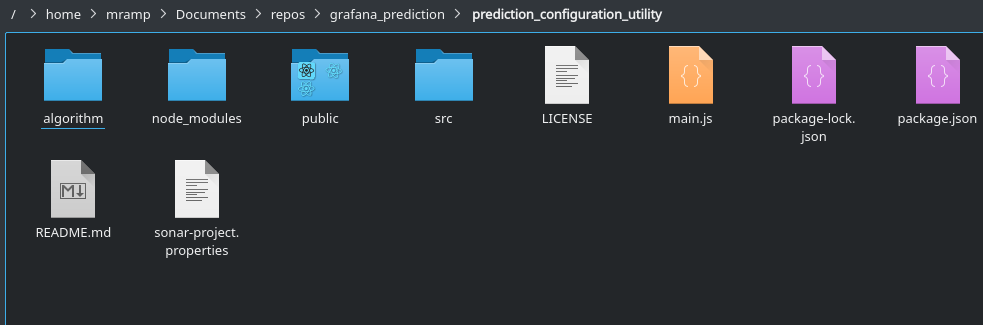
\includegraphics[width=\textwidth,height=\textheight,keepaspectratio]{img/directoryProject.png}
	\end{center}
	\caption{Selezione app nella directory}	
\end{figure}



\subsubsection{Installare le dipendenze}%\mbox{}\\ [1mm]
Per il corretto funzionamento dell'applicazione è necessario installare tutte le dipendenze elencate nel file \texttt{package.json}. Per farlo, eseguire da terminale nella cartella \verb|prediction_configuration_utility| il comando:
\begin{verbatim}
	npm install
\end{verbatim}
I pacchetti che vengono installati si suddividono in dipendenze e dipendenze sviluppatore.
%\\
%\\POCO VISIBILE
%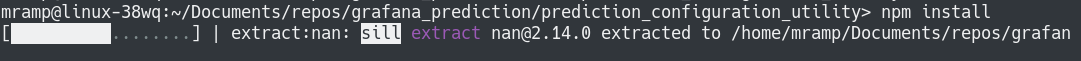
\includegraphics[width=\textwidth,height=\textheight,keepaspectratio]{img/packageInstallation.png}

\paragraph*{Dipendenze}\mbox{}\\ [1mm]
Nella seguente tabella sono elencate tutte le dipendenze necessarie per la corretta esecuzione dell'applicazione.
\mbox{}\\ [1mm]
\rowcolors{2}{gray!25}{gray!15}
	\setcounter{table}{0}
	\begin{longtable} {
		>{}p{65mm} 
		>{}p{30mm}
		}
    \rowcolor{gray!50}
    \textbf{Pacchetto} & \textbf{Versione} \TBstrut \\ [2mm]
    \verb|@testing-library/jest-dom| & \verb|^4.2.4|  \TBstrut \\ [2mm]
    \verb|@testing-library/react| & \verb|^9.3.2| \TBstrut \\ [2mm]
    \verb|@testing-library/user-event| & \verb|^7.1.2| \TBstrut \\ [2mm]
    \verb|csvtojson| & \verb|2.0.10| \TBstrut \\ [2mm]
    \verb|d3| & \verb|^5.15.0| \TBstrut \\ [2mm]
    \verb|electron-is-dev| & \verb|^1.1.0| \TBstrut \\ [2mm]
    \verb|ml-modules|\footnote{Il pacchetto \texttt{ml-modules} usato nel nostro progetto è una versione modificata dell'ononimo pacchetto} & \verb|0.1.0| \TBstrut \\ [2mm]
    \verb|react| & \verb|^16.13.0| \TBstrut \\ [2mm]
    \verb|react-dom| & \verb|^16.13.0| \TBstrut \\ [2mm]
    \verb|react-router-dom| & \verb|^5.1.2| \TBstrut \\ [2mm]
    \verb|react-scripts| & \verb|3.4.0| \TBstrut \\ [2mm]
    \rowcolor{white}
    \caption{Dipendenze per eseguire applicazione}
    \end{longtable}
    
\paragraph*{Dipendenze sviluppatore}\mbox{}\\ [1mm]
Nella seguente tabella sono elencate tutte le dipendenze necessarie per la corretta esecuzione dell'applicazione durante lo sviluppo della stessa.
\rowcolors{2}{gray!25}{gray!15}
	\setcounter{table}{0}
	\begin{longtable} {
		>{}p{65mm} 
		>{}p{30mm}
		}
    \rowcolor{gray!50}
    \textbf{Pacchetto} & \textbf{Versione} \TBstrut \\ [2mm]
    \verb|electron| & \verb|^8.02| \TBstrut \\ [2mm]
    \verb|electron-packager| & \verb|^14.2.1| \TBstrut \\ [2mm]
    \verb|coveralls| & \verb|^3.0.9| \TBstrut \\ [2mm]
    \verb|enzyme| & \verb|^3.11.0| \TBstrut \\ [2mm]
    \verb|enzyme-adapter-react-16| & \verb|^1.15.2| \TBstrut \\ [2mm]
    \verb|spectron| & \verb|^10.0.1| \TBstrut \\ [2mm]
    \rowcolor{white}
    \caption{Dipendenze specifiche per lo sviluppatore}
    \end{longtable}
    \mbox{}\\ [1mm]
Seguendo i due passaggi descritti nei precedenti paragrafi, l'applicazione esterna è installata correttamente.

\subsection{Installazione ambiente di sviluppo integrato WebStorm}
Per installare l'ambiente di sviluppo integrato WebStorm, visitare la pagina \url{https://www.jetbrains.com/webstorm/download/}. Qui è possibile trovare il download per MacOS, Windows e sistemi operativi basati su Linux/Unix.
\\
%\\
%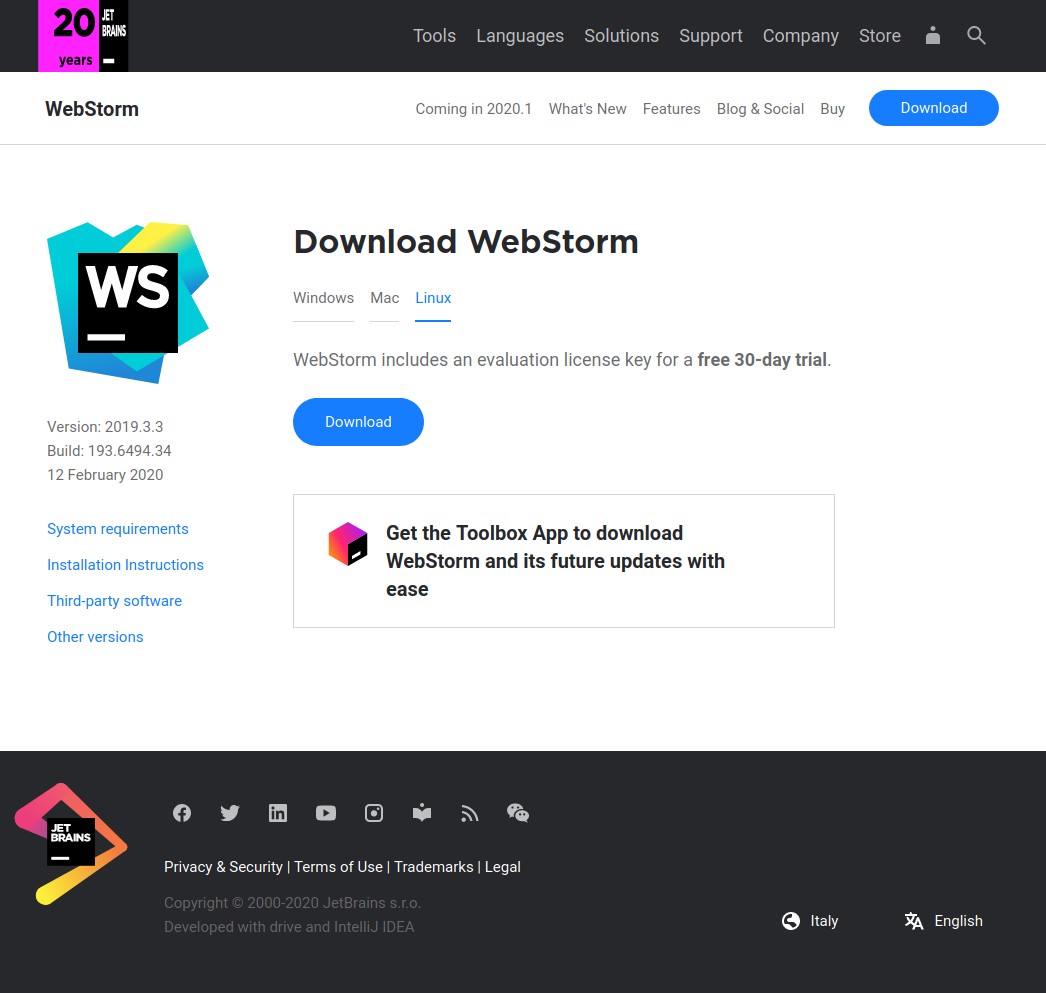
\includegraphics[width=\textwidth,height=\textheight,keepaspectratio]{img/webstorm.png}

%\pagebreak
\subsubsection{Installazione plug-in SonarLint per WebStorm}
Per installare il plug-in SonarLint per WebStorm, aprire le impostazioni di WebStorm dal suo menù "File". Quindi nella sezione "Plugins" cercare ed installare "SonarLint".
\\
\\
\begin{figure}[H] 	
	\begin{center}
		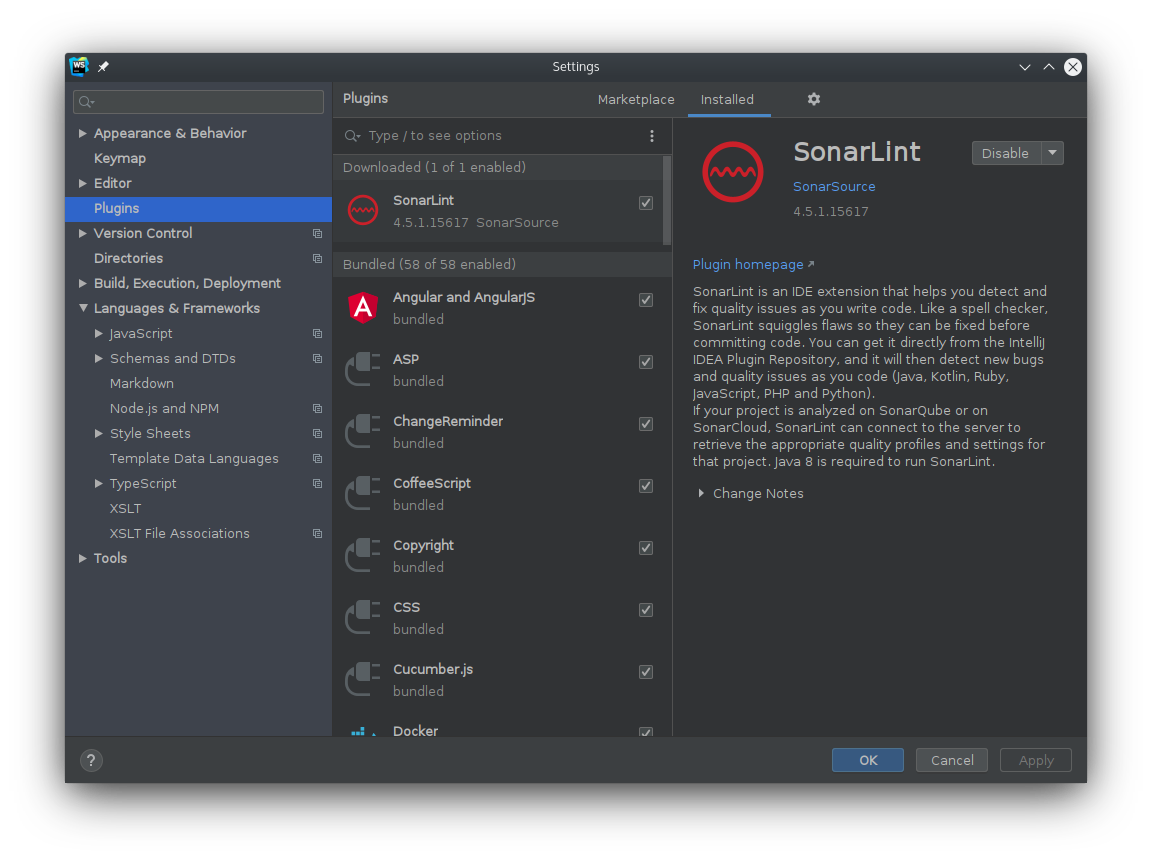
\includegraphics[width=\textwidth,height=\textheight,keepaspectratio]{img/sonarlint.png}
	\end{center}
	\caption{Installazione SonarLint}	
\end{figure}

